\chapter{Aνάπτυξη ηλεκτρονικών παιχνιδιών}
Aνάπτυξη ηλεκτρονικών παιχνιδιών (game development) ονομάζουμε τη διαδικασία της δημιουργίας ενός παιχνιδιού. Η ομάδα ανάπτυξης μπορεί να κυμαίνεται από ένα άτομο μέχρι μια μεγάλη επιχείρηση.	
	\subsection{Ιστορική αναδρομή}
	Η ιστορία των βιντεοπαιχνιδιών, αρχίζει στα τέλη της δεκαετίας του '40. Προς τα τέλη του '50 και στα μέσα του '60, στην Αμερική, αρχίζουν να μπαίνουν στην καθημερινή ζωή οι υπολογιστές, για την ακρίβεια, οι κεντρικοί υπολογιστές. Από εκείνη την περίοδο, τα βιντεοπαιχνίδια έκαναν την εμφάνισή τους, στις κονσόλες, στα φλίπερ, στους υπολογιστές, αλλά και στις φορητές κονσόλες. Από τότε η δημιουργία παιχνιδιών έχει γιγαντωθεί έχοντας ένα τεράστιο κομμάτι της παγκόσμιας οικονομίας.
	Πλέον ο ανταγωνισμός είναι τεράστιος, τα βιντεοπαιχνίδια κυκλοφορούν με πολύ γρήγορο ρυθμό, για διάφορες κονσόλες, με πολύ απαιτητικά γραφικά.
			
	\section{Ανάπτυξη παιχνιδιών}
	Η ανάπτυξη παιχνιδιών περιλαμβάνει πολλές εξειδικευμένες ειδικότητες, οι οποίες παράγουν μια μηχανή γραφικών.
	
	\subsection{Μηχανές γραφικών}	
	Στο τομέα του σχεδιασμού παιχνιδιών το πιο διαδεδομένο CASE tool είναι η μηχανή γραφικών. Μια μηχανή γραφικών είναι μια σουίτα από επαναχρησιμοποιήσιμα οπτικά εργαλεία, τα οποία βρίσκονται σε ένα ενιαίο περιβάλλον.
	Η κεντρική λειτουργικότητα η οποία παρέχεται περιλαμβάνει τη φωτοαπόδοση σε πραγματκό χρόνο (real time rendering), τη μηχανή φυσικής και εντοπισμό συγκρούσεων (physics and collision detection), το scripting, το animation, την τεχνητή νοημοσύνη (Artificial Intelligence), τη δικτύωση (networking), τον παραλληλισμό ενεργειών (multitasking), την διαχείριση μνήμης και τον γράφο σκηνής (scene graph). Η ανάπτυξη των παιχνιδιών μέσω μιας μηχανής γραφικών γίνεται εύκολα, γρήγορα και οδηγούμενη από δεδομένα (data driven), ούτως ώστε οι δημιουργοί παιχνιδιών να έχουν την ευχέρεια να επικεντρώνονται στις λεπτομέρειες του παιχνιδιού τους.
	Οι μηχανές αναπτύσσονται από ομάδες που απαρτίζονται όχι μόνο από προγραμματιστές, αλλά και από μαθηματικούς, φυσικούς κλπ. Η κάθε υποομάδα εστιάζει σε ένα συγκεκριμένο υποσύστημα. Για παράδειγμα οι φυσικοί ασχολούνται με τον εντοπισμό συγκρούσεων, ενώ οι αρχιτέκτονες λογισμικού ασχολούνται με τη σύνδεση και αλληλεπίδραση των υποσυστημάτων σε υψηλό επίπεδο, χωρίς να τους απασχολούν οι λεπτομέρειες υλοποίησης του κάθε υποσυστήματος.
	
	\subsection {Τι είναι μια μηχανή γραφικών}
	Η πρώτη αναφορά σε μηχανή γραφικών έγινε στα μέσα της δεκαετίας του 90 και αναφερόταν στο δημοφιλές παιχνίδι Doom, του οποίου η αρχιτεκτονική διαχώριζε τα βασικά συστήματα του παιχνιδιού, όπως τη φωτοαπόδοση (rendering system), τον εντοπισμό συγκρούσεων (collision detection system), το υποσύστημα ήχου (audio system), το υποσύστημα διαχείρισης πόρων (resource management system) κλπ. Η αξία αυτού του διαχωρισμού εκτιμήθηκε από την κοινότητα όταν οι προγραμματιστές ξεκίνησαν να πουλάνε άδειες για το λογισμικό και επαναχρησιμοποιούσαν εργαλεία προηγούμενων παιχνιδιών με δημιουργία νέων assets. Μικρότερα στούντιο τροποποιούσαν εκδόσεις υπάρχοντων παιχνιδιών χρησιμοποιώντας το \gls{SDK}.
	Πολλά παιχνίδια γράφτηκαν με σκοπό την επαναχρησιμοποίηση κώδικα και \gls{modding}. Πολλές μηχανές, όπως η μηχανή του Quake III, γράφτηκαν με τρόπο ώστε να είναι εύκολα προσαρμόσιμες χρησιμοποιώντας scripting και με σκοπό την εμπορευματοποίηση μέσω αδειοδότησης (licensing).
	Η διαχωριστική γραμμή μεταξύ του παιχνιδιού και της μηχανής δεν μπορεί να οριστεί με ακρίβεια. Πολλές μηχανές μπορεί να περιέχουν συγκεκριμένα μέρη, που αφορούν συγκεκριμένη λειτουργία του παιχνιδιού. Η μεγάλη διαφορά είναι η οδηγούμενη από δεδομένα αρχιτεκτονική (data-driven architecture) όπου οι κανόνες και τα στοιχεία δεν είναι σκληρά κωδικοποιημένα (hard coded), αλλά διαβάζονται από εξωτερικό αρχείο.
	Τα χαρακτηριστικά και τα όρια των μηχανών ορίζονται ανάλογα με το είδος του παιχνιδιού στο οποίο η μηχανή εστιάζει και με βάση τις πλατφόρμες και τις κάρτες γραφικών στις οποίες προορίζεται η ανάπτυξη. Για παράδειγμα η \gls{OpenGLES} η οποία χρησιμοποιείται από τα κινήτα είναι υποσύνολο της \gls{OpenGL} και δεν υποστηρίζει όλες τις λειτουργίες της \gls{OpenGL} \cite{opengleslimitations}.
	
	\subsection{Γιατί να χρησιμοποιήσει κάποιος μηχανή γραφικών;}	
	Η αφαίρεση πάντα βοηθούσε τον εγκέφαλο να λειτουργήσει καλύτερα και να κατανοήσει αλληλεπιδράσεις μεταξύ συστημάτων και περίπλοκες έννοιες. Οι μηχανές γραφικών απαλλάσσουν τους γραφίστες και τους προγραμματιστές από τις τεχνικές λεπτομέρειες, και εστιάζουν στην αισθητική και στο gameplay. Επίσης με την αποσύνδεση των συστημάτων έχουμε πιο προβλέψιμη συμπεριφορά, επεκτασιμότητα των υποσυστημάτων ως υποσυστήματα και εύκολη δοκιμαστικότητα (testability).
	
\subsection{Δομή μιας μηχανής γραφικών}
Η μοντελοποίηση της δομής των μηχανών γραφικών σε αφαιρετικό επίπεδο είναι πανομοιότυπη, διαφέρει όμως η υλοποίηση. Η δομή ξεκινά να διαφοροποιείται στα υψηλότερα επίπεδα, τα οποία υλοποιούνται με στόχο το σχεδιασμό συγκεκριμένου είδους παιχνιδιών. Μια τυπική μηχανή γραφικών παρουσιάζεται στην εικόνα \ref{fig:Game_Engine_Architecture} \cite{gregory2009game}.
	\begin{figure}
		\centering
		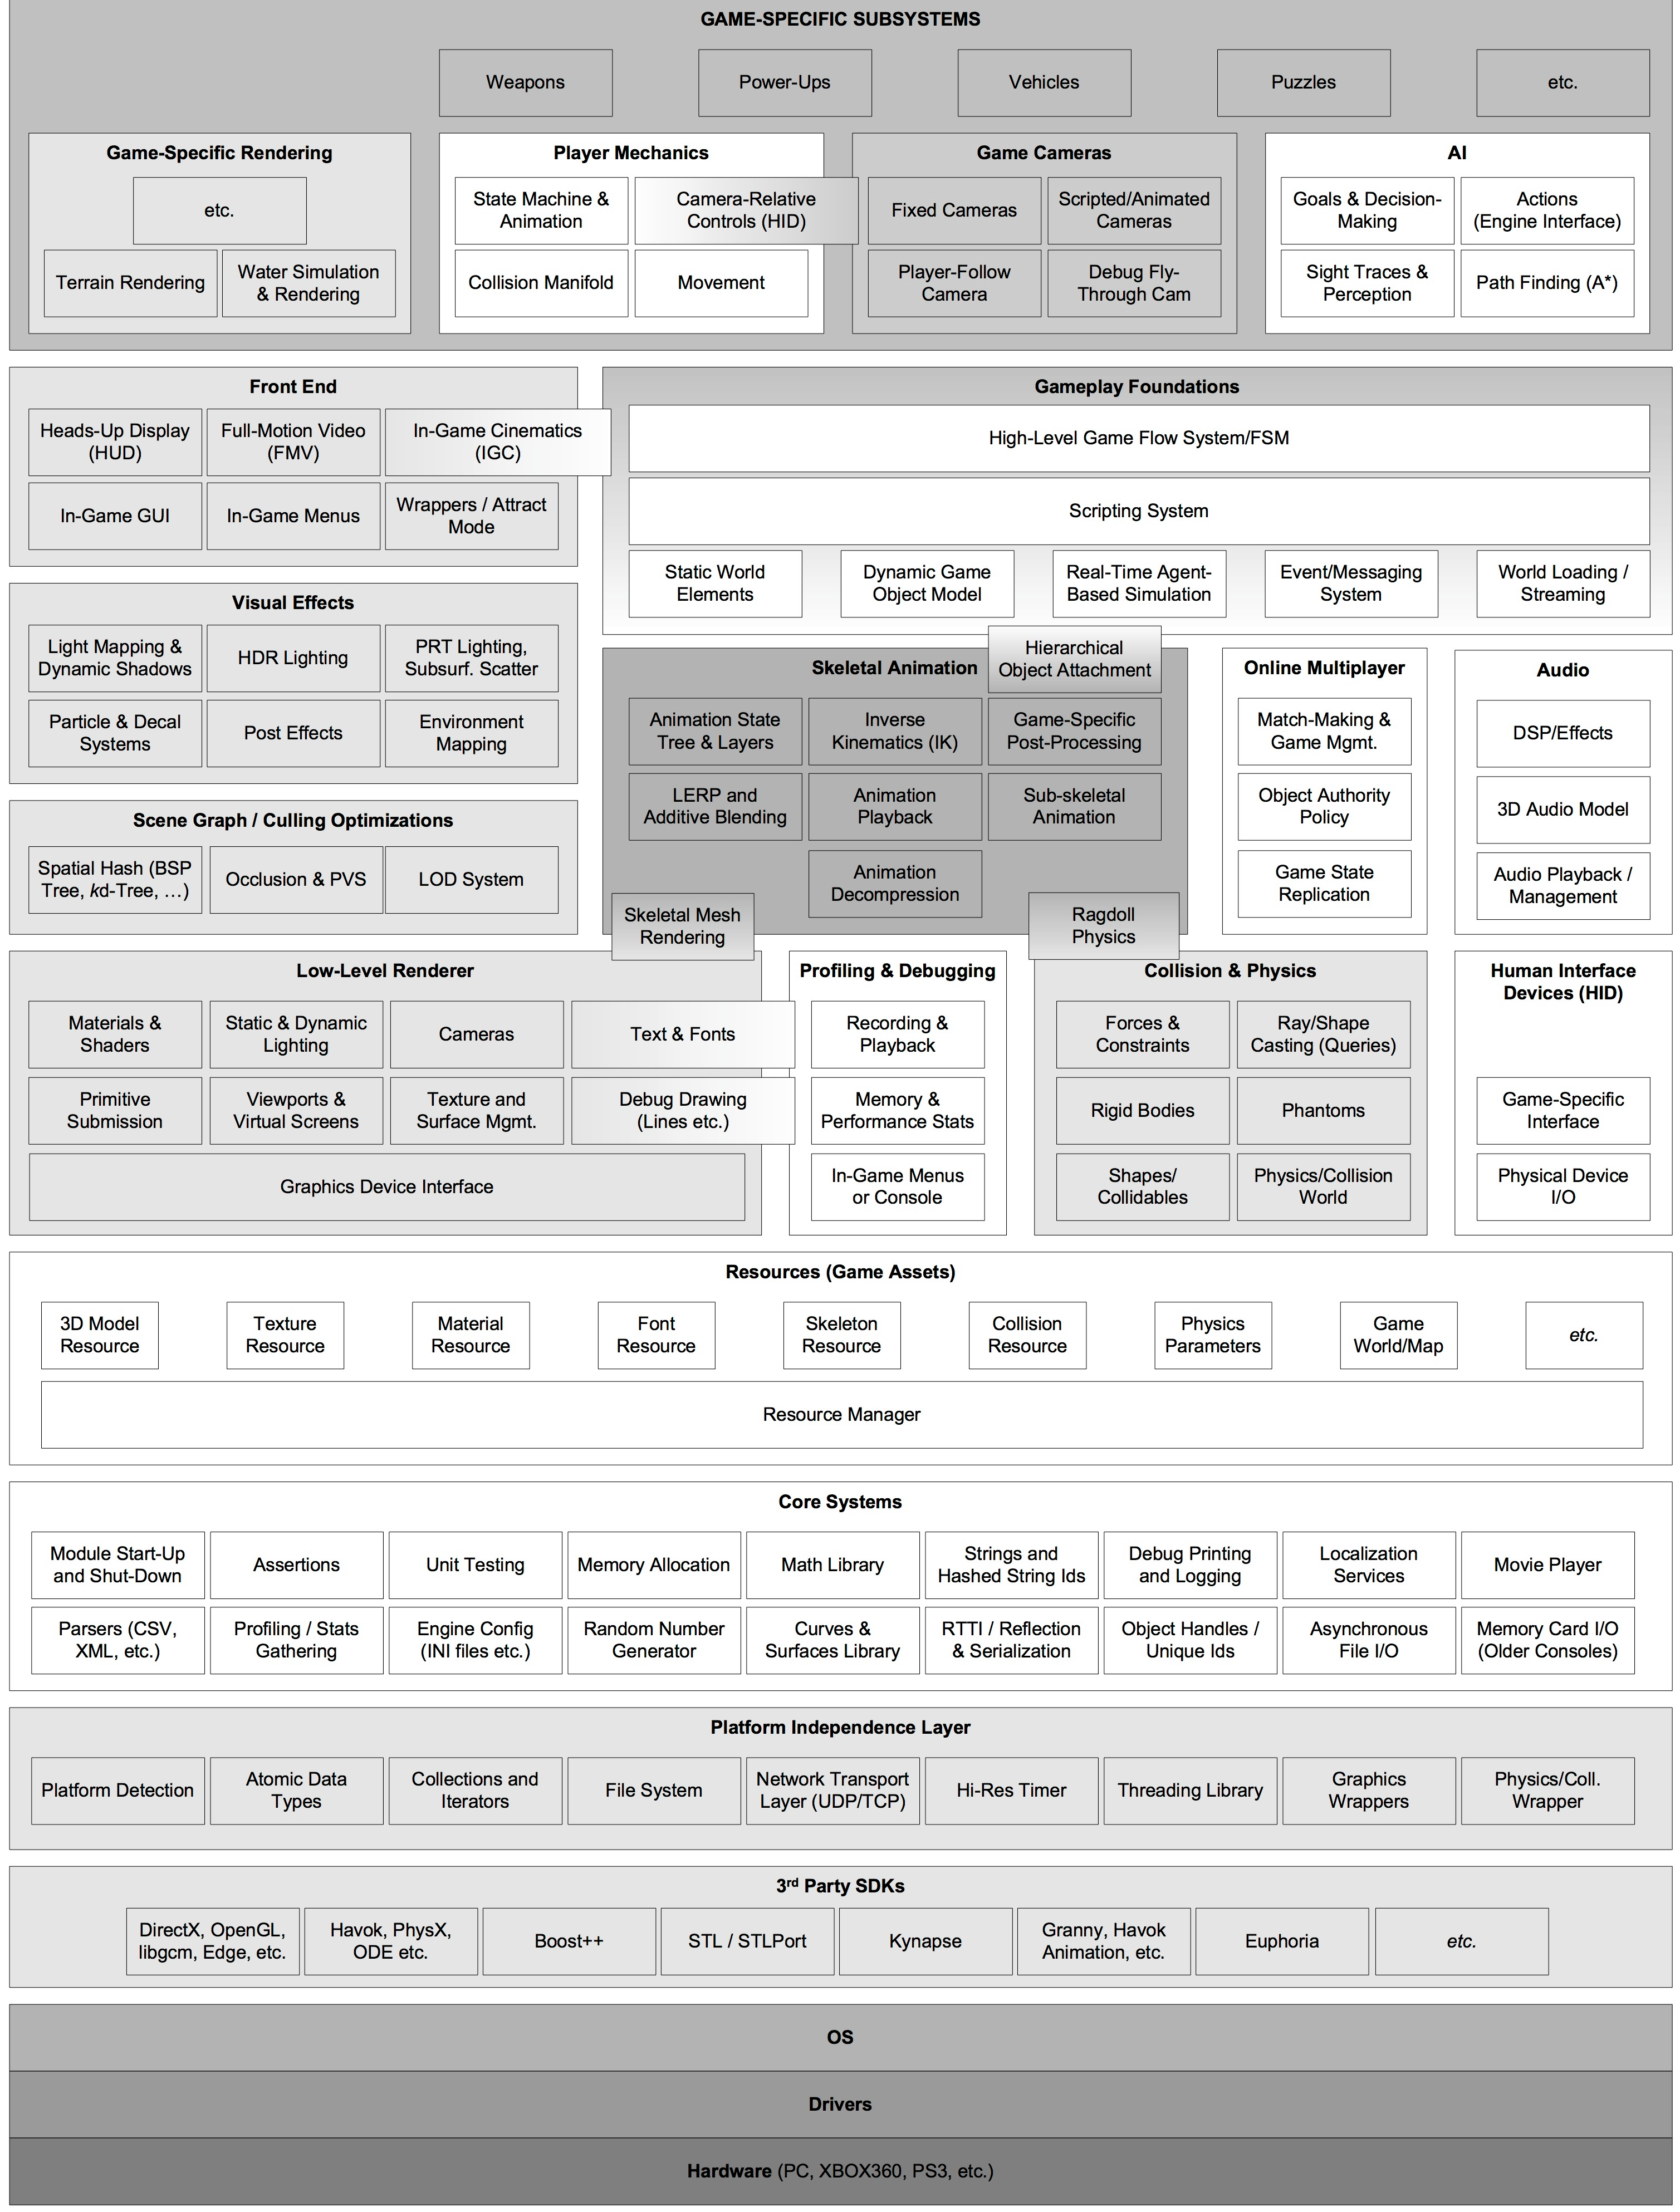
\includegraphics[width=160mm]{Images/game_engine_architecture}
		\caption{Τυπική αρχιτεκτονική μηχανής γραφικών}
		\label{fig:Game_Engine_Architecture}
	\end{figure}	

\paragraph{Επισκόπηση επιπέδων της μηχανής γραφικών}
\begin{description}	
\item [Υλισμικό]Το υλισμικό (hardware) αντιπροσωπεύει το υλικό στο οποίο θα τρέξει το παιχνίδι, δηλαδή τον υπολογιστή ή την κονσόλα.

\item [Οδηγοί]Οι οδηγοί (drivers) διαχειρίζονται τους πόρους του υλικού και του λειτουργικού και παρέχουν ένα καθολικό πρωτόκολλο επικοινωνίας μεταξύ των διαφόρων παραλλαγών.

\item [Λειτουργικό Σύστημα]Το λειτουργικό σύστημα είναι ο ενορχηστρωτής των προγραμμάτων. Κατανέμει το χρόνο μεταξύ των πόρων του υλικού και των προγραμμάτων και παραλληλίζει την εκτέλεση των προγραμμάτων. Στις κονσόλες το λειτουργικό παίζει τυπικό ρόλο, αφού το λογισμικό (παιχνίδια) έχει σχεδόν πλήρη έλεγχο του υλικού. Πλέον όμως στις σύγχρονες κονσόλες και στα λειτουργικά συστήματα όπως Microsoft Windows, κανένα πρόγραμμα δεν έχει πλήρη έλεγχο, αφού το λειτουργικό μπορεί να μοιραστεί πόρους του συστήματος με το τρέχον λογισμικό για να εμφανίσει για παράδειγμα κάποιο μήνυμα.

\item [Third party SDKs and Middleware]Πολλές φορές χρησιμοποιούνται βιβλιοθήκες ανάπτυξης λογισμικού τρίτων, οι οποίες γράφτηκαν από την κοινότητα και λύνουν κοινά προβλήματα. Συχνό παράδειγμα είναι η χρήση βιβλιοθηκών για δομές δεδομένων, η για απόδοση (rendering).

\item [Εντοπισμός συγκρούσεων]Εντοπισμός συγκρούσεων και δυναμική άκαμπτου σώματος (rigid-body dynamics) δηλαδή το πώς ένα σύστημα με διασυνδεδεμένα σώματα αντιδρά όταν του ασκούνται εξωτερικές δυνάμεις.

\item [Ανεξαρτησία πλατφόρμας]Πολλά παιχνίδια καλούνται να τρέξουν σε περισσότερες από μία πλατφόρμες. Στο επίπεδο ανεξαρτησίας πλατφόρμας (platform independence layer) οι εντολές του λειτουργικού σύστηματος  και υλικού ενθυλακώνονται (encapsulated) για να μπορούν να αλλάξουν ανάλογα με το περιβάλλον ανάπτυξης.

\item [Συστήματα Πυρήνα]Κάθε μεγάλο και σύνθετο πρόγραμμα χρειάζεται κάποιες βιβλιοθήκες γενικής χρήσης. Κάποιες από αυτές είναι: 

	\begin{description}
	\item [Ισχυρισμοί]	Ισχυρισμούς (assertions) ονομάζουμε τα κομμάτια κώδικα, τα οποία ελέγχουν τις υποθέσεις του προγραμματιστή, για το πώς πρέπει να εκτελεστεί η συνάρτηση. Ο κώδικας αυτός αφαιρείται στις τελικές εκδόσεις, αφού περάσει η περίοδος δοκιμών.
	
	\item [Διαχείριση μνήμης]Στο σύστημα διαχείρισης μνήμης (memory management) γίνεται έλεγχος της μνήμης για αποφυγή θρυμματισμού (fragmentation) και συνθήκες μη διαθέσιμης μνήμης (out of memory).
	
	\item [Βιβλιοθήκη μαθηματικών]Η βιβλιοθήκη μαθηματικών περιέχει μαθηματικά, τα οποία χρειάζονται στις προσομοιώσεις πραγματικού χρόνου, όπως είναι τα διανύσματα, οι πίνακες, η γεωμετρία κλπ.
	\end{description}

\item [Διαχείριση πόρων]Το υποσύστημα διαχείρισης πόρων (resource management) ασχολείται με τη διαχείριση των πόρων του παιχνιδιού, όπως τα μοντέλα, τα textures, ο κόσμος, οι χάρτες κλπ.

\item [Μηχανή απόδοσης] Η μηχανή απόδοσης (rendering engine) είανι το πιο σύνθετο κομμάτι της μηχανής, το οποίο είναι υπεύθυνο για την αναπαράσταση του παιχνιδιού στην οθόνη.
 
\item [Απόδοση χαμηλού επιπέδου]Η απόδοση χαμηλού επιπέδου (low-level renderer) εστιάζει στην βελτιστοποίηση των πρωτογενών γεωμετρικών σχημάτων.

\item [Γράφος σκηνής]Ο γράφος σκηνής (scene graph) καθορίζει ποια αντικείμενα πρέπει να αποδοθούν (render) από τη μηχανή απόδοσης (rendering engine), χρησιμοποιώντας αλγόριθμους ανάλογα με το μέγεθος και το είδος του παιχνιδιού.

\item [Οπτικά εφέ] Τα οπτικά εφέ (visual effects) αποτελούνται από το σύστημα σωματιδίων (particle system), τη χαρτογράφηση φωτός (light mapping), τις δυναμικές σκιές (dynamic shadows), το anti-aliasing κλπ.
 
\item [Front End]Front end ονομάζεται το επίπεδο επικοινωνίας με το παιχνίδι, όπως το μενού, η κονσόλα, τα pop-ups παράθυρα κλπ.

\item [Profiling and Debugging]Η ποιότητα της απόδοσης του παιχνιδιού είναι πολύ κρίσιμη. Για να γίνει βελτιστοποίηση της απόδοσης, χρειάζονται εργαλεία ανάλυσης του υλικού στο οποίο τρέχει το παιχνίδι με οπτική αναπαράσταση.

\item [Σύστημα συγκρούσεων και φυσικής]Η φυσική και οι συγκρούσεις (physics and collision) είναι στενά συνδεδεμένες γιατί οι συγκρούσεις επιλυόνται με κανόνες φυσικής.

\item [Animation]Animation είναι η ταχεία προβολή μιας σειράς από εικόνες (δισδιάστατης ή τρισδιάστατης μακέτας) ή θέσεων ενός μοντέλου, έτσι ώστε να δημιουργείται η ψευδαίσθηση της κίνησης.

\item [Συσκευές ανθρώπινης διεπαφής]Οι συσκευές ανθρώπινης διεπαφής (human interface devices) είναι βιβλιοθήκες για έλεγχο των σημάτων από το πληκτρολόγιο, το ποντίκι, τα χειριστήρια, τα οποία χρησιμοποιεί ο χρήστης για να επικοινωνήσει με το παιχνίδι. Επίσης πολλές φορές χρησιμοποιούνται για να επικοινωνήσει το παιχνίδι με το χρήστη, όπως η δόνηση στο χειριστήριο.

\item [Ήχος]Το σύστημα διαχείρισης ήχου έχει πολλές δυνατότητες. Μπορεί να χρησιμοποιηθεί για τρισδιάστατη αναπαράσταση του ήχου, για να δώσει την αίσθηση του βάθους και της απόστασης στον χρήστη.

\item [Δικτύωση]Συνήθως ένας χρήστης παίζει μόνος του σε ένα εικονικό κόσμο. Πολλές φορές όμως άλλοι χρήστες συνδέονται σε αυτό τον κόσμο μέσω online multilayer.

\item [Gameplay Foundation Systems]Στο gameplay foundation system ορίζονται οι κανόνες του εικονικού κόσμου, οι οποίοι οριοθετούν τις δυνατότητες του παίχτη.

\item [Game Worlds and Object Models]Η αναπαράσταση του κόσμου με αντικειμενοστραφή τρόπο (game object model) περιλαμβάνει το στατικό background, τη δυναμική στερεών σωμάτων (dynamic rigid bodies), τους παίχτες (player characters), τους non-player characters, τα όπλα, τα οχήματα, τον φωτισμό, τις κάμερες κλπ.

\item [Σύστημα συμβάντων]To σύστημα συμβάντων (event system) είναι το σύστημα το οποίο επιτρέπει την επικοινωνία του μοντέλου αντικειμένου παιχνιδιού (game object model) με τον εαυτό του.

\item [Scripting System]To scripting σε μία μηχανή γραφικών, επιταχύνει την ανάπτυξη γιατί περιέχει χρήσιμες, συχνές και έτοιμες προς εκτέλεση εντολές.

\item [Τεχνητή νοημοσύνη]Η τεχνητή νοημοσύνη (artificial intelligence) περιλαμβάνει τυπικά patterns νοημοσύνης, όπως την πλοήγηση (navigation), την εύρεση διαδρομής (path finding), τη δυναμική αποφυγή αντικειμένων (dynamic object avoidance) κλπ.

\item [Game Specific Subsystems]Game specific subsystems ονομάζουμε τα συστήματα τα οποία βρίσκονται σε πιο ψηλά επίπεδα από τη μηχανή γραφικών και αφορούν το παιχνίδι το οποίο αναπτύσσεται.

\item [Tools and Asset Pipeline]Όλα τα παιχνίδια χρειάζονται πολλά δεδομένα για να αναπαραστήσουν τον εικονικό κόσμο, όπως τη διαμόρφωση (configuration), τα scripts, τα τρισδιάστατα μοντέλα κλπ. Οι μηχανές πρέπει να είναι σε θέση να επεξεργάζονται συγκεκριμένου τύπου δεδομένα τα οποία εξάγονται από δημοφιλή προγράμματα δημιουργίας ψηφιακού περιεχομένου ( digital content creation programs).

\item [Βάση δεδομένων πόρων]Η βάση δεδομένων πόρων (resource database) υλοποιεί τεχνικές αναζήτησης και αποθήκευσης των πόρων του παιχνιδιού. Χρησιμοποιούνται από υπάρχουσες βάσεις δεδομένων, μέχρι \gls{XML} αρχεία. 
\end{description}

\section{Σχεδιασμός παιχνιδιών}
Σχεδιασμό παιχνιδιών (game design) ονομάζουμε τον σχεδιασμό και την εφαρμογή τεχνικών αισθητικής στη δημιουργία ενός παιχνιδιου με σκοπό τη διευκόλυνση της αλληλεπίδρασης μεταξύ των παικτών. Οι μηχανές γραφικών χρησιμοποιούνται για σκοπούς δημιουργίας παιχνιδιών (game design). Οι σχεδιαστές παιχνιδιών (game designers) σχεδιάζουν το πώς θα είναι το παιχνίδι χωρίς να τους απασχολούν οι τεχνικές λεπτομέρειες. Είναι υπεύθυνοι για:
\begin{itemize}
	\item Τα εργαλεία και μηχανισμούς μέσα στο παιχνίδι
	\item Την ανάπτυξη κανόνων
	\item Την ιστορία και πλοκή
	\item Την στρατηγική και την τυχαιότητα	
\end{itemize}

Όπως και το game engineering, το game design χωρίζεται σε υποκατηγορίες και τεχνικές. Οι κατηγορίες αυτές διαφέρουν ανάλογα με το μέγεθος της ομάδας και το παιχνίδι το οποίο σχεδιάζεται.

	\subsection{Μοντέλο MDA}
	Στo μοντελο \gls{MDA} ο σχεδιασμός παιχνιδιών χωρίζεται στη μηχανική (mechanics), δυναμική (dynamics) και αισθητική (aesthetics).
	\cite{mda04}.
	
	\begin{description}
	\item [Μηχανική] Μηχανική ονομάζουμε τα διάφορα συστατικά ενός παιχνιδιού, στο επίπεδο αλγορίθμων και της αναπαράστασης.
	\item [Δυναμική] Δυναμική είναι η συμπεριφορά των mechanics κατά τον χρόνο εκτέλεσης, αντιδρώντας στις εισόδους και εξόδους του συστήματος με την πάροδο του χρόνου
	\item [Αισθητική] Αισθητική ονομάζουμε τις επιθυμητές συναισθηματικές αντιδράσεις τις οποίες προκαλεί η συσκευή αναπαραγωγής όταν αλληλεπιδρά με τον παίχτη.	
	\end{description}

\subsection{Πως ορίζεται ένα παιχνίδι}
Διαισθητικά ο καθένας μπορεί να ξεχωρίσει τι είναι ένα παιχνίδι όπως το σκάκι και η μονόπολη. Στη θεωρία παιχνιδιών, ένα παιχνίδι είναι ένα σύνολο παραγόντων οι οποίοι δρουν βάση στρατηγικών και τεχνικών, με στόχο να μεγιστοποιήσουν τα κέρδη μέσα στον εικονικό κόσμο, μέσα σε ένα πλαίσιο καλά ορισμένων κανόνων.

Ο Raph Koster στο βιβλίο του a Theory of Fun for Game Design \cite{koster04}, ορίζει το παιχνίδι ως μια διαδραστική εμπειρία, η οποία παρέχει στον χρήστη μια προκλητική σειρά από πρότυπα (patterns) τα οποία μαθαίνει και στην τελική εξειδικεύεται. Ισχυρίζεται ότι η εκμάθηση και εξειδίκευση βρίσκονται στην καρδιά του τι θεωρείται διασκεδαστικό, όπως ένα λογοπαίγνιο γίνεται αστείο τη στιγμή που ο εγκέφαλος αντιληφθεί το πρότυπο (pattern).

Στο βιβλίο The Grasshopper του Bernand Suits  \cite{suits2005grasshopper}. καθηγητή φιλοσοφίας στο πανεπιστήμιο του Waterloo, δηλώνει ότι "ένα παιχνίδι είναι η εθελοντική προσπάθεια να ξεπεραστούν περιττά εμπόδια".
O Tracy Fullerton στο βιβλίο του Game Design Workshop \cite{fullerton2008game} ορίζει ένα παιχνίδι ως "ένα κλειστό, σύστημα που δεσμεύει τους παίκτες σε ένα δομημένο περιβάλλον σύγκρουσης και επιλύει την αβεβαιότητά του με ένα άνισο αποτέλεσμα. Oι ορισμοί είναι επηρεασμένοι από το περιβάλλον και τις προθέσεις των συγγραφέων, είναι όμως σωστοί με το δικό τους τρόπο.

\section{Δομή μιας τυπικής ομάδας ανάπτυξης παιχνιδιών}
	Πριν από την ανάλυση της δομής της μηχανής, θα γίνει ανάλυση της δομής της ομάδας η οποία θα χρησιμοποιεί τη μηχανή, για να αναπτυχθούν στοχευμένα εργαλεία για το κάθε πρόβλημα της κάθε υποομάδας.
	
	\paragraph{Μηχανικοί}	
	Οι μηχανικοί σχεδιάζουν και υλοποιούν το λογισμικό του παιχνιδιού και τα εργαλεία τα οποία χρησιμοποιούνται για την ανάπτυξή του. Οι δύο μεγάλες κατηγορίες μηχανικών είναι οι
	\begin{description}
		\item [Runtime programmers] Οι runtime programmers ασχολούνται με τη μηχανή και το παιχνίδι.
		\item [Προγραμματιστές εργαλείων] Οι προγραμματιστές εργαλείων γράφουν εργαλεία τα οποία αυτοματοποιούν και ευκολύνουν τη διαδικασία ανάπτυξης.
	\end{description}
	Οι μηχανικοί έχουν είτε κάποια ειδικότητα, για παράδειγμα ειδικότητα στη τεχνητή νοημοσύνη, είτε είναι generalists, δηλαδή κατέχουν από όλα τα στοιχεία και μπορούν να λύσουν προβλήματα που προκύπτουν κατά τη διάρκεια ανάπτυξης.
	
	\paragraph{Καλλιτέχνες}
	Οι καλλιτέχνες (artists) παράγουν όλο το οπτικοακουστικό κομμάτι του παιχνιδιού, το οποίο είναι βασικό κομμάτι για το χαρακτήρα του παιχνιδιού. Χωρίζονται στις εξής κατηγορίες
	
	\begin{description}
		\item [Concept artists] 
		Οι concept artists σχεδιάζουν σκίτσα και πίνακες τα οποία παρέχουν στην ομάδα την εικόνα του τελικού παιχνιδιού. Παρέχουν οπτική καθοδήγηση στην ομάδα καθ' όλη τη διάρκεια του κύκλου ανάπτυξης.
		\item [3D Modelers]
	    Οι 3D modelers είναι υπεύθυνοι για την τρισδιάστατη γεωμετρία του εικονικού κόσμου του παιχνιδιού. Απαρτίζονται από τους
		foreground modelers οι οποίοι σχεδιάζουν χαρακτήρες, οχήματα, όπλα και αντικείμενα του τρισδιάστατου κόσμου
		background modelers οι οποίοι σχεδιάζουν το στατικό περιβάλλον πχ κτήρια.
		\item [Texture artists] Οι texture artists σχεδιάζουν τις δισδιάστατες εικόνες που καλύπτουν τα τρισδιάστατα μοντέλα
		\item [Lighting artists] Οι lighting artists ορίζουν τις στατικές και δυναμικές πηγές φωτός και δουλεύουν με το χρώμα και την κατεύθυνση του φωτός.
		\item [Animators] Οι animators σχεδιάζουν την κίνηση των χαρακτήρων και των αντικειμένων
		\item [Hθοποιοί σύλληψης κίνησης] Οι ηθοποιοί σύλληψης κίνησης (motion capture actors) παρέχουν ακατέργαστα δεδομένα κίνησης για να επεξεργαστούν οι animators και να τα ενσωματώσουν στο παιχνίδι.
		\item [Sound designers] Οι sound designers παράγουν τα εφέ και τη μουσική.
		\item [Voice actors] H φωνή των voice actors ηχογραφείται και χρησιμοποιείται για τους χαρακτήρες στο παιχνίδι.
	\end{description}
	
	\paragraph{Σχεδιαστές}
	Η δουλειά ενός σχεδιαστή παιχνιδιών (game designer) είναι να σχεδιάσει το διαδραστικό τμήμα του παιχνιδιού, το gameplay. Ασχολούνται με τον σχεδιασμό επιπέδων, την ιστορία, τις αλληλεπιδράσεις μεταξύ των χαρακτήρων στο παιχνίδι, με τους στόχους, σκοπούς και κανόνες του παιχνιδιού.
	Σχεδιάζουν το κάθε επίπεδο μοναδικά και αποφασίζουν για τη γεωμετρία στο περιβάλλον, πότε και πού εμφανίζονται χαρακτήρες και διάφορα αντικείμενα, πώς γίνονται οι μεταβάσεις μεταξύ διάφορων σκηνών κλπ.
	
	\paragraph{Παραγωγοί}
	Ο ρόλος του παραγωγού (producer) διαφέρει από στούντιο σε στούντιο. Η βασική του δουλειά είναι να προγραμματίζει και να δρομολογεί τις διάφορες εργασίες και να λειτουργεί ως ο συνδετικός κρίκος μεταξύ των ατόμων που παίρνουν ηγετικές αποφάσεις και την ομάδα ανάπτυξης. Οι producers είναι χαρακτηριστικό των μεγάλων εταιριών, όπου υπάρχουν πολλά τμήματα και πολλοί εργαζόμενοι.	
	
